
%%%%%%%%%%%%%%%%%%%%%%%%%%%%%%%%%%%%%%
\section{Teorie: Signalizační protokol SIP}
\label{sip}
Session Initiation Protocol (SIP, RFC 3261, červen 2002) je textový aplikační protokol pro signalizaci VoIP, který provádí:
\begin{itemize}
    \item vytváření a udržování relace
    \item adresování pomocí SIP URI sip:user@domain
    \item registace uživatele
    \item navazování spojení, směrování hovorů
\end{itemize}

\noindent SIP {\bf neprovádí} správu relací po jejich navázání, nezajišťuje kvalitu přenosu a nezajišťuje přenos hlasových dat. \\
~\\
\noindent {\bf Základními prvky} jsou server UAS (User Agent Server) a uživatelský agent UAC (User Agent Client). UAS může mít více úloh,
např. registrační (přijímá žádosti REGISTER), proxy (analyzuje zprávy, směruje hovory), lokalizační (informace o umístění klientů)
nebo server pro směrování (další bod spojení – hop – u altern. SIP serveru). \\
~\\
\noindent {\bf Adresování} používá SIP URI ve tvaru sip:user@domain, např. sip:matousp@cesnet.cz. {\bf Směrovací informace} uloženy v SIP
hlavičce paketu Via, Route, Record-Route. {\bf Směrování} provádí servery SIP na cestě.

\subsection*{Příklad signalizace SIP}
\begin{lstlisting}
INVITE sip:541141118@cesnet.cz SIP/2.0
Call-ID: D40CA785-2EEE-4801-9B04-349632F56CDC@147.229.14.146
CSeq: 2 INVITE
From: "Petr Matousek"<sip:matousp@cesnet.cz>;tag=2007034328740
To: <sip:541151118@cesnet.cz>

SIP/2.0 100 Trying -- your call is important to us
Call-ID: D40CA785-2EEE-4801-9B04-349632F56CDC@147.229.14.146
CSeq: 2 INVITE
From: "Petr Matousek"<sip:matousp@cesnet.cz>;tag=2007034328740
To: <sip:541151118@cesnet.cz>
\end{lstlisting}

\subsection*{Základní metody protokolu SIP}
\begin{itemize}
    \item REGISTER – žádost o registraci
    \item INVITE, ACK, CANCEL – vytváření spojení
    \item BYE – ukončení spojení
    \item OPTIONS – zjišťování možností přenosu
    \item PRACK – provizorní ACK
\end{itemize}

\subsection*{Další metody protokolu SIP}
\begin{itemize}
    \item INFO (RFC 6086) – přenost aplikačních inforpací
    \item MESSAGE (RFC 3428) – textové zprávy IM
    \item SUBSCRIBE, NOTIFY (RFC 3265) – zasílání upozornění na události
    \item PUBLISH (RFC 3903) – zveřejnění stavu událostí (prezence)
\end{itemize}

\subsection*{Položky hlavičky SIP}
\begin{itemize}
    \item {\bf Via} - Obsahuje směrovací informace. Každý server, přes který SIP zpráva po cestě projde,
    přidá do hlavičky jeden řádek Via s IP adresou a číslem portu, na kterém zpracoval paket. Odpověď v opačném
    směru pak prochází shora dolů všemi servery, které jsou uvedené ve Via. Každý server zpracuje paket,
    odstraní svůj vlastní záznam a odešle ho na následující adresu ve Via. Poslední záznam Via je IP adresa
    a číslo portu klienta.
    \begin{figure}[h!]
        \centering
        \fbox{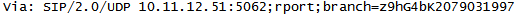
\includegraphics[width=125mm]{img/via.png}}
    \end{figure}
    
    \item {\bf From} - Adresa odesílatele SIP zprávy. Obsahuje SIP URI a nepovinně zobrazitelné jméno (display-name).
    Display-name (zde {\tt user03}) je určeno pouze pro „lidského uživatele“.
    U registrace obsahuje pole From SIP URI adresu uživatele, který je zodpovědný za registraci. Pokud se nejedná o registraci třetí strany, je hodnota stejná jako To.
    \begin{figure}[h!]
        \centering
        \fbox{
\includegraphics[width=95mm]{img/from.png}}
    \end{figure}

    
    \item {\bf To} - Adresa příjemce zprávy. Může to být koncový uživatel nebo adresa SIP proxy (next hop), která zpracuje danou žádost.
    U registrace je v To uvedena adresa uživatele, která má být na serveru zaregistrována nebo modifikována.
    \begin{figure}[h!]
        \centering
        \fbox{
\includegraphics[width=43mm]{img/to.png}}
    \end{figure}
    
    \item {\bf Allow} - Seznam SIP metod, které daný uživatel podporuje a používá.
    \begin{figure}[h!]
        \centering
        \fbox{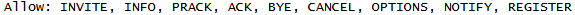
\includegraphics[width=135mm]{img/allow.png}}
    \end{figure}
\end{itemize}

\subsection*{SDP}
Session description protocol (SDP) se používá pro zaslání informací potřebných pro přijímání hlasového toku.
Nepřenáší se pomocí něj vlastní data, slouží pro vyjednání parametrů, jako je typ média (video, audio, atd.),
transportní protokol (RTP/UDP/IP, H.320, atd.), typ kodeku nebo přenosová rychlost.
SDP zprávy se přenáší ve zprávách SIP typu INVITE a OK. \\
~\\
\noindent Příklad zprávy SDP:
\begin{lstlisting}
v=0                                             # version
o=- 3434794301 3434794301 IN IP4 147.229.14.146 # originator
s=Sjphone                                       # session name
c=IN IP4 147.229.14.146                         # address
t=0 0 # time (start + end)
a=direction:passive
m=audio 49152 RTP/AVP 3 97 98 8 0_101           # media stream
a=rtpmap:3 GSM/8000
a=rtpmap:97 iLBC/8000
a=rtpmap:98 iLBC/8000
a=fmtp:98 mode=20
a=rtpmap:8 PCMA/8000
a=rtpmap:0 PCMU/8000
a=rtpmap:101 telephone-event/8000
a=fmtp:101 0-11,16
\end{lstlisting}
